% \documentclass[12pt, twoside]{article}
\usepackage[letterpaper, margin=1in, headsep=0.2in]{geometry}
\setlength{\headheight}{0.6in}
%\usepackage[english]{babel}
\usepackage[utf8]{inputenc}
\usepackage{microtype}
\usepackage{amsmath}
\usepackage{amssymb}
%\usepackage{amsfonts}
\usepackage[nomessages]{fp} %\FPeval{\var-name}{2*sin(pi/6)}
\usepackage{siunitx} %units in math. eg 20\milli\meter
\usepackage{yhmath} % for arcs, overparenth command
\usepackage{tikz} %graphics
\usetikzlibrary{quotes, angles, arrows, arrows.meta}
\usepackage{graphicx} %consider setting \graphicspath{{images/}}
\usepackage{parskip} %no paragraph indent
\usepackage{enumitem}
\usepackage{multicol}
\usepackage{venndiagram}

\usepackage{fancyhdr}
\pagestyle{fancy}
\fancyhf{}
\renewcommand{\headrulewidth}{0pt} % disable the underline of the header
\raggedbottom
\hfuzz=2mm %suppresses overfull box warnings

\usepackage{hyperref}

\fancyhead[LE]{\thepage}
\fancyhead[RO]{\thepage \\ Name: \hspace{4cm} \,\\}
\fancyhead[LO]{BECA / Dr. Huson / Geometry\\*  Unit 4: Volume and polyhedra \\* 19 October 2022}

\begin{document}

\subsubsection*{4.7 Homework: Mixed area and volume practice}
  \begin{enumerate}
  \item Find the area of $\triangle RAT$. The altitude $h$ of the triangle is 2.7 centimeters and the base $RA=5.4$ cm. Show work by writing an equation before making the calculation.
    \begin{flushright}
    \begin{tikzpicture}[scale=0.9, rotate=20]
      \draw [thick]
        (2,0)node[below]{$R$}--
        (8,0)node[below]{$A$}--
        (4,3)node[above]{$T$} --(2,0);
    \draw [dashed] (4,0)--(4,3);
    \draw (4,0)++(0.3,0)--++(0,0.3)--+(-0.3,0);
    \node at (4,1.2)[right]{$h=2.7$};
    \node at (5,-0.2)[below]{$5.4$};
    \end{tikzpicture}
    \end{flushright} \vspace{1.0cm}

  \item Find the area of the parallelogram $ABCD$ shown below, with $AB=40$ millimeters and height $h=24$ mm.
    \begin{flushright}
    \begin{tikzpicture}[scale=0.8]
      \draw [-, thick] (0,0)--(5,0)--(6,3)--(1,3)--cycle;
      \draw [-, dashed] (5,0)--(5,3);
      \draw [fill] (0,0) circle [radius=0.05] node[left]{$A$};
      \draw [fill] (5,0) circle [radius=0.05] node[right]{$B$};
      \draw [fill] (6,3) circle [radius=0.05] node[right]{$C$};
      \draw [fill] (1,3) circle [radius=0.05] node[left]{$D$};
      \node at (4.3, 1.5){$24$};
      \node at (2.5, -0.5){40 mm};
    \end{tikzpicture}
    \end{flushright} \vspace{1.0cm}

  \item  A wooden cutting board is $11 \frac{1}{4}$ inches long, 8 inches wide, and $1 \frac{1}{2}$ inches thick. Find the volume of wood in cubic inches. \hfill (\textbf{diagram not to scale})
    \begin{flushright}
      \begin{tikzpicture}[scale=1]
        \draw [-, thick] (0,0)--(7,0)--(7,1)--(0,1)--cycle;
        \draw [-, thick] (0,1)--(0.5,2.5)--(7.5,2.5)--(7,1);
        \draw [-, thick] (7,0)--(7.5,1.5)--(7.5,2.5);
        \node at (7.8, 2){$1 \frac{1}{2}$};
        \node at (3.5, -0.35){$11 \frac{1}{4}$};
        \node at (7.6, 0.8){$8$};
      \end{tikzpicture}
      \end{flushright} \vspace{2cm}

\newpage
\subsubsection*{Model the situation with an equation. Use the formula sheet on the last page. You must start with a labeling variable. \hfill Do NOT solve!}

\item \emph{Worked example:} Find the radius of a circle circumference of 14.7.
\[C=2\pi r=14.7\]

\item A prism has a base area of 20 square centimeters. Its volume is 200 cubic centimeters. Find the prism's height, $h$. \vspace{2cm}

\item A water tank in the shape of a cylinder has a volume of 250 cubic feet. Its height is 12 feet. Find the radius of the base of the tank. \vspace{2cm}

\item A spherical cork fishing net float has a volume of 4000 cubic centimeters. Find its radius. \vspace{2cm}

\item The volume of a cone having a \textbf{diameter} of 10 inches is 200 cubic inches. Find the cone's height. \vspace{2cm}

\item The volume of the Great Pyramid of Giza, the tomb of Pharoah Khufu, is approximately 2,500,000 cubic meters. It is 140 meters tall. Find the area of its base.  \vspace{2cm}

\item The smaller pyramid for his wife, Queen Meretites, has a square base with an area of 2500 square meters. Find the length of the side of its base, $s$.

\newpage
\item In your notebook, write the formulas for the area and circumference of circles:
\[A=\pi r^2\]
\[C=\pi D = 2\pi r\]

  \item Given the circle centered at $O$ with radius $r=4$.
  \begin{multicols}{2}
    \begin{enumerate}
      \item Find the circumference of a circle. %\vspace{1cm}
      \item Find the area of the circle.\vspace{3cm}
    \end{enumerate}
    %\columnbreak
    \begin{tikzpicture}[scale=.635]
      \draw [help lines] (-5,-5) grid (5,5);
      %\draw [thick, ->] (-2.2,0) -- (10.4,0) node [below right] {$x$};
      %\draw [thick, ->] (0,-2.2)--(0,10.4) node [left] {$y$};
      \draw (0,0) circle [radius=4] node[below]{$O$};
      \draw [fill] (0,0) circle [radius=0.05];
    \end{tikzpicture}
  \end{multicols}

  \item Given the semi-circle shown with diameter $AB=6$. Find its area and perimeter.
    \begin{flushright}
    \begin{tikzpicture}[scale=.635]
      \draw [help lines] (-5,-1) grid (5,4);
      \draw [thick] (-3,0)node[below left]{$A$} -- (3,0)node[below right]{$B$};
      %\draw [thick, ->] (0,-2.2)--(0,10.4) node [left] {$y$};
      \draw [thick] (3,0) arc (0:180:3);
      \draw [fill] (-3,0) circle [radius=0.05];
      \draw [fill] (3,0) circle [radius=0.05];
    \end{tikzpicture}
  \end{flushright} \vspace{1cm}

  \item Find the radius of a circle having an area of $25 \pi$. \vspace{2cm}
  \item Find the diameter of a circle with a circumference of 31.416.


\end{enumerate}
\end{document}